\documentclass[17pt,hyperref={pdfpagelabels=false}]{beamer}
\usetheme{Berlin}
\usecolortheme[light,accent=blue]{solarized}
\usepackage{booktabs}
\usepackage{lmodern}
\usepackage{listings}
\usepackage{color}
\usepackage{graphicx}
\usepackage{fancybox}
\usepackage[orientation=landscape,size=a0,scale=1.4]{beamerposter}
\setbeamertemplate{headline}{\hfill{}}
\setbeamertemplate{navigation symbols}{}

% Lengths and such
\newlength{\onecolumnwidth}
\setlength{\onecolumnwidth}{0.31\paperwidth}

\graphicspath{{figures/}}
\title{OpenCUDA+MPI}
\subtitle{A Framework for Heterogeneous GP-GPU Cluster Computing}
\author[Ballou, Mousa]{Kenny Ballou, Nilab Mohammad Mousa}
\institute[Boise State]{College of Engineering, Department of Computer Science,
Boise State University}
\date[Aug. 2nd, 2013]{August 2nd, 2013}
\begin{document}
\begin{frame}[t]
\begin{block}{}
\Huge{\textcolor{solarizedAccent}{OpenCUDA + MPI}}\hfill{}\\{}
\huge{A Framework for Heterogeneous GP-GPU Computing}\hfill{}\\{}
\large{Kenny Ballou, Boise State University Department of Computer
Science\hfill{}\\{}
Nilab Mohammad Mousa, Boise State University Department of Computer
Science\hfill{}\\{}
Mentor: Alark Joshi, PhD. Boise State University Department
of Computer Science\hfill{}\\{}}
\end{block}

\begin{columns}[t,onlytextwidth=\textwidth]
    \begin{column}{0.99\paperwidth}
        \begin{columns}[t,onlytextwidth=\textwidth]
        \begin{column}[t,onlytextwidth=\textwidth]{\onecolumnwidth}
            \begin{block}{\Large Abstract}
The introduction and rise of General Purpose Graphics Computing has
significantly impacted parallel and high-performance computing. It has
introduced challenges when it comes to distributed computing with GPUs. Current
solutions target specifics: specific hardware, specific network topology, a
specific level of processing. Those restrictions on GPU computing limit
scientists and researchers in various ways. The goal of OpenCUDA+MPI project is
to develop a framework that allows researchers and scientists to write a
general algorithm without the overhead of worrying about the specifics of the
hardware and the cluster it will run against while taking full advantage of
parallel and distributed computing on GPUs. As work toward the solution
continues to progress, we have proven the need for the framework and expect to
find the framework enables scientists to focus on their research.
\end{block}

            \begin{block}{\Large Project Objectives}
\begin{itemize}
\item{Develop a framework for highly-parallel computation, utilizing many GPU's
over many computers}
%\begin{itemize}
%\item{Framework shall lower entry costs into high performance computing}
%\end{itemize}
\item{Provide cluster administration tools and configurations}
\item{Framework and related code shall be Free and Open-Source software}
\end{itemize}
\end{block}

            \begin{block}{\Large Methodology}
To fully understand the purpose of creating a framework, we first set out to
attempt developing parallel code \emph{without} our proposed framework.

We also want to not only compare times of development speed, but actual running
time of each solution. As such, we developed a CPU only, a single GPU, and a
distributed GPU solution to the N-Body problem and compared running times of
each for several different problem sizes.\hfill{}\\{}

The N-Body problem was chosen as a test problem because it is \emph{not}
an embarassingly parallel problem and, as such, requires inter-communication.
\end{block}

        \end{column}
        \begin{column}[t,onlytextwidth=\textwidth]{\onecolumnwidth}
            % vim: syntax=tex:
\section{Results}

\subsection{Vector Summation}

Our first developed test program was a $ 10 $ billion element wise vector
summation problem. This is a simple and, as we will see, a bad example of using
a cluster to speed up the computational time required. Although we did see a
increase in performance, the cost of \gls{io} far out weighs the benefit.
Specifically, to do the computation on one machine (one \gls{cpu}), it took a
\gls{wall_time} of $254$ seconds (about $4$ minutes) and a \gls{cpu_time} of
$13.7$ seconds.  Further, to do the computation using a single \gls{gpu} took
about $4172$ seconds (\gls{wall_time}) or about $70$ minutes, $13.83$ seconds
(\gls{cpu_time}) while the computing the summation of the cluster took about
$3177$ seconds (\gls{wall_time}) or about $50$ minutes, $10.51$ seconds
(\gls{cpu_time}). Our \gls{cpu} only implementation took the least amount of
elapsed time, it took the second longest \gls{cpu_time}. Our \gls{cuda} only
implementation took the longest in both \gls{wall_time} and \gls{cpu_time} and
our cluster implementation was shortest \gls{cpu_time} but seconds longest
elapsed time. The benefit of saving an upwards of $3.3$ seconds is not worth
the extra incurred cost of $2923$ seconds. Not so surprisingly though, running
the vector summation problem over the cluster \emph{without} using \gls{cuda}
does increase the overall elapsed time of the problem; namely, it took $226$
seconds \gls{wall_time} (currently the correct \gls{cpu_time} is unable to be
collected). Further, increasing the number of nodes part of the program's pool,
decreases the \gls{wall_time} for each node.

\begin{table}[htb]
\centering{}
\begin{tabular}{lcc}
\toprule{}
\textbf{Method} & \textbf{Time (s)} & \textbf{Total Time (s)} \\
\midrule{}
CPU Only & 13.7 & 254.13 \\
\midrule{}
CUDA (Single \Gls{node}) & 13.83 & 4172 \\
\midrule{}
MPI + CUDA (7 \glspl{node}) & 10.51 & (average) 3177 \\
\midrule{}
MPI (7 \glspl{node}) & & (average) 226  \\
\midrule{}
MPI (16 \glspl{slot}) & & (average) 149 \\
\bottomrule{}
\end{tabular}
\caption{Computational Timing Comparison of $ 10^9 $ element wise vector
summation}
\end{table}

\subsection{N-Body Problem}

We have several sizes of the \texttt{N-Body} problem that we tested with:
$2,001$ particles, $20,000$ particles, $200,000$ particles, $2,000,000$, and
$20,000,000$ particles.\\

The computational times are for only one time step. The method for computing
the gravitational potential is an adaptation of the \gls{p3m} method. The
benefit of using this method is we are able to nicely distribute the problem
over the \gls{cluster} and / or over a \gls{gpu} (because of memory
limitations) while maintaining a respectable accuracy for close body
interactions. Further, if a grid contains more bodies than a specified
threshold (in our case $200,000$), we can further sub-divide the grid to
improve performance and maintain accuracy still.\\

There are other algorithms for computing \texttt{N-Body} problems on the
\gls{cpu} that are quite efficient, notably, the Barnes-Hut Tree
algorithm\cite{barneshut1986}; however, using it would distort and confound the
comparisons between \gls{cpu}, \gls{gpu}, and \gls{cluster} implementations,
not to mention the complexities of implementing such an algorithm on
\glspl{gpu} and over a \gls{cluster}.

\subsubsection{N-Body --- CPU}

In \gls{cpu} tests, we were only able to complete several of the problem sizes;
the larger sizes are infeasible. Notably, the smaller sizes were computed in a
relatively respectable amount of time. While the bigger sizes were time
consuming, not even attempted, or aborted. For example, the 2 million body
problem was aborted after running for about 2 weeks.

\begin{table}[htb]
\centering{}
\begin{tabular}{lccc}
\toprule{}
\textbf{Size} & \textbf{User (seconds)} &
\textbf{Sys (seconds)} & \textbf{Real (seconds)} \\
\midrule{}
2001          & 28.81   & 0.02    & 30.77   \\
\midrule{}
20000         & 2382.40 & 2.27    & 2393    \\
\midrule{}
200000        & 113983  & 34.45   & 114349  \\
\midrule{}
2 million     & aborted & aborted & aborted \\
\midrule{}
20 million    & N/A     & N/A     & N/A     \\
\bottomrule{}
\end{tabular}
\caption{\gls{cpu} N-Body simulation using particle-particle method}
\label{tab:cpu_nbody}
\end{table}

\subsubsection{N-Body --- GPU}

As noted above, the \gls{gpu} (\gls{cuda}) implementation uses the same
computational method (\gls{p3m}). Using the \gls{gpu}, we were able to compute
the $ 20,000,000 $ size problem and may be able to compute larger sets within a
\emph{reasonable} amount of time. See \cref{tab:gpu_nbody} for a breakdown of
the running times.

\begin{table}[htb]
\centering{}
\begin{tabular}{lccc}
\toprule{}
\textbf{Size} & \textbf{User (seconds)} &
\textbf{Sys (seconds)} & \textbf{Real (seconds)} \\
\midrule{}
2001          & 10.08   & 1.52    & 14.14  \\
\midrule{}
20000         & 22.30   & 2.46    & 26.82  \\
\midrule{}
200000        & 44.63   & 4.84    & 52.86  \\
\midrule{}
2 million     & 186.59  & 21.23   & 217.60 \\
\midrule{}
20 million    & 1289.24 & 159.29  & 1510   \\
\bottomrule{}
\end{tabular}
\caption{Single \gls{gpu} (\gls{cuda}) N-Body simulation using \gls{p3m}
method}
\label{tab:gpu_nbody}
\end{table}

\subsubsection{N-Body --- 16 Node Cluster}

Similar to the other solutions, we are still using the \gls{p3m} method for
computing a single time step of the N-Body problem. Over 16 nodes, we were able
to see drastic improvements over \gls{cpu} and \gls{cuda} implementations.
Notably, in the $20,000$ problem size, the \gls{cluster} did nearly $19044\%$
better than the \gls{cpu} and about $115\%$ better than a single \gls{gpu}.
Further, in the $200,000$ problem size, we see the \gls{cluster} did about
$535,743\%$ better versus \gls{cpu} and about $148\%$ better versus \gls{gpu}.
See \cref{tab:cudampi_nbody} for times of each problem size.

\begin{table}[htb]
\centering{}
\begin{tabular}{lccc}
\toprule{}
\textbf{Size} & \textbf{User (seconds)} &
\textbf{Sys (seconds)} & \textbf{Real (seconds)} \\
\midrule{}
2001          & N/A     & N/A      & N/A     \\
\midrule{}
20000         & 0.17    & 0.032    & 12.50   \\
\midrule{}
200000        & 0.147   & 0.028    & 21.34   \\
\midrule{}
2 million     & 0.15    & 0.025    & 97.76   \\
\midrule{}
20 million    & 0.15    & 0.06     & 950.045 \\
\bottomrule{}
\end{tabular}
\caption{16 node \gls{cluster} N-Body simulation using \gls{p3m} method}
\label{tab:cudampi_nbody}
\end{table}

            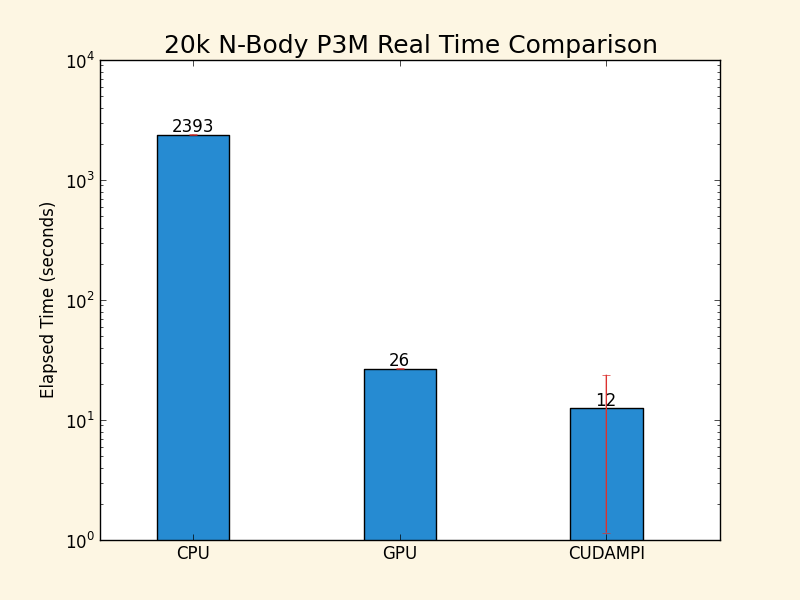
\includegraphics[scale=0.9]{20k_bar_chart.png}
            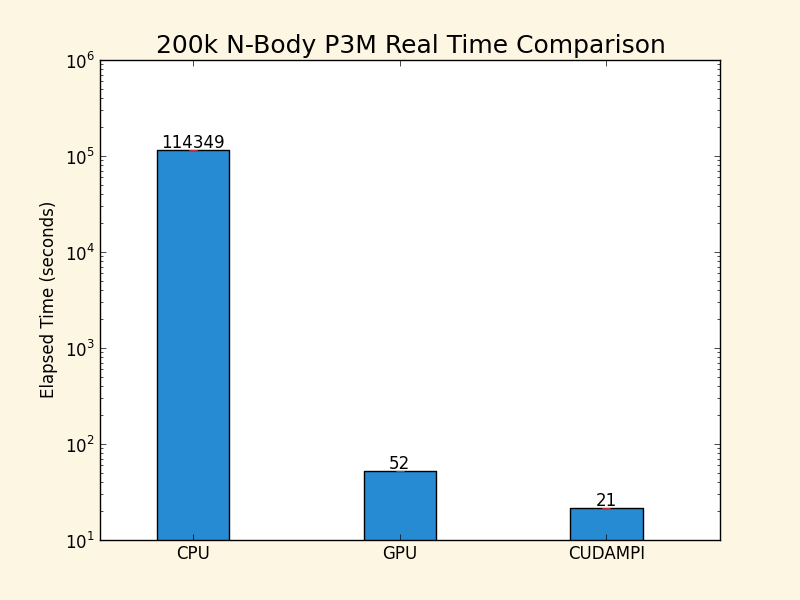
\includegraphics[scale=0.9]{200k_bar_chart.png}
            \hfill{}\\{}
            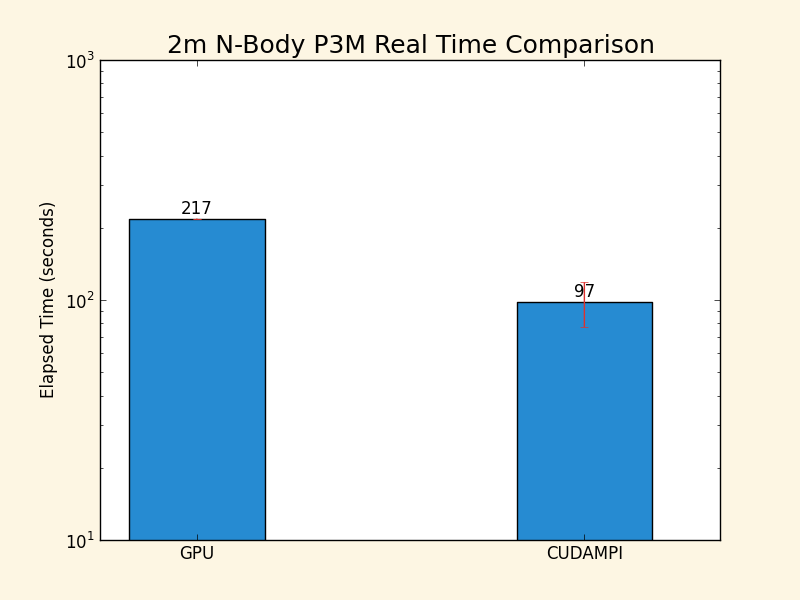
\includegraphics[scale=0.9]{2m_bar_chart.png}
            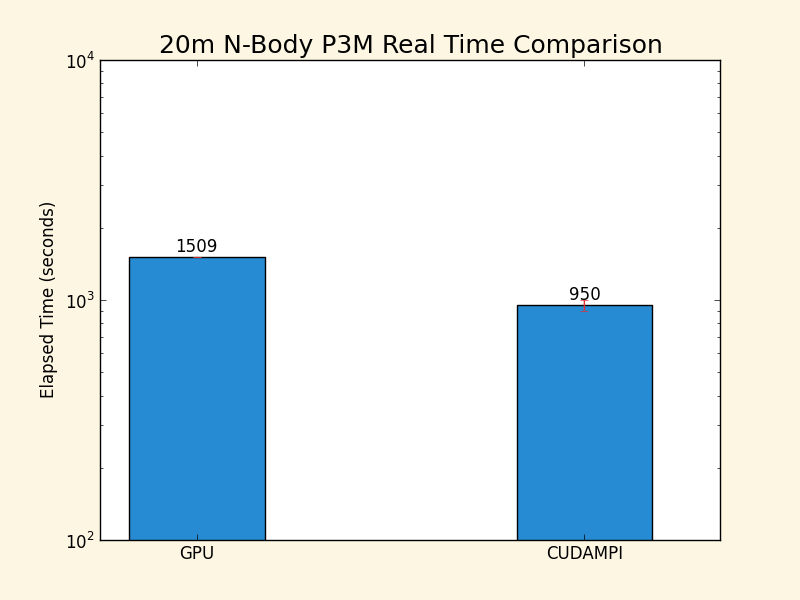
\includegraphics[scale=0.9]{20m_bar_chart.png}
        \end{column}
        \begin{column}[t,onlytextwidth=\textwidth]{\onecolumnwidth}
            \begin{block}{\Large Conclusions and Discussion}
We can clearly see the increase in performance when we distribute our work over
many machines. If our problem is particularly I/O bound, however, we may be
causing more slow downs or bottlenecks than worth the computational performance
increase.\hfill{}\\{}

We need to test the framework more, and with more, different problems. Doing so
would highlight areas that need adjustment or re-working. Further, it would
show the framework's viability to others and in other problem spaces.
\end{block}

            \begin{block}{\Large Future Work}
\begin{itemize}
\item{Add better debugging, logging and profiling to the framework}
\item{Expose control of CUDA device initilaization}
\item{Add automatic/ configurable checkpointing}
\item{(Finish) Node Configuration}
\begin{itemize}
\item{Master/ Head Node Configuration}
\item{Add real (job) scheduler}
\end{itemize}
\end{itemize}
\end{block}

            % vim: syntax=tex:
\section{Acknowledgements}

We would like to take this opportunity to thank everyone that helped and made
this project a possibility. Thanks to the Student Research Initiative
Fellowship for providing the motivation and funding. Lastly (and certainly not
least), a special thanks to our mentor, Alark Joshi, PhD., giving us the
high-level guidance and inspiration when it mattered most.

            \vspace{1cm}
            
\includegraphics[scale=0.8]{bsulogo.png}\hspace{1cm}
            
\includegraphics[scale=0.5]{nvidia-cuda2.png}\hspace{1cm}
            
\includegraphics[scale=1.0]{open-mpi-logo.png}\hspace{1cm}
            
\includegraphics[scale=0.2]{python.png}
        \end{column}
        \end{columns}
    \end{column}
\end{columns}
\end{frame}
\end{document}
